\section{A decidable case $d=2$}
\label{sec:2d}
\subparagraph*{Reaching $\mu\Phi$ with optimal choice.}
Before finally focusing on the case~$d=2$, we provide useful reasoning steps valid in arbitrary dimension.
Let~$\mathcal{S}$ be generated by matrices~$M_1, \dots, M_r$.

As evident from~\cref{eps-pre-fp}, 
it is not sufficient to have a matrix~$M$ with $M\cdot \eps(\bm{x}) = \bm{0}$,
in order for~$\mu\Phi$ to be reachable from~$\bm{x}$ in one iteration of~$\Phi$.
The Bellman operator makes an optimal choice from the set of matrices,
and multiplication with the chosen matrix has to yield the fixed point.
	For later discussions, it is convenient to define a new operator~$F$ as
	\[F(\bm{v}) = \max_{1\leq i \leq r} \left(M_i \cdot\bm{v}\right).\]
	Clearly, for the iterative application of~$F$, it holds $F^n(\bm{v}) = \max_{1\leq i_1, \dots, i_n \leq r} \left(M_{i_n}\dots M_{i_1} \cdot\bm{v}\right))$.
	Using~\cref{eps-facts}, we note $\eps(\Phi^n(\bm{x})) = F^n(\eps(\bm{x}))$.
	Therefore, the BOR problem can be concisely formulated as deciding whether $F^n(\eps(\bm{s})) = \bm{0}$ for some~$n \geq 0$.

\begin{definition}
	The \emph{$F$-preimage $F^{-1}(\bm{0})$ of the zero vector} 
is the set of all vectors~$\eps$ such that $F(\eps) = \bm{0}$.
Equivalently, $F^{-1}(\bm{0})$ 
is the set of all $\eps:=\eps(\bm{x})$ such that $\Phi(\bm{x}) = \mu\Phi$.
\end{definition}
\begin{remark}\label{preim-phi}
	The set~$F^{-1}(\bm{0})$ is entirely contained in the union of all kernels~$\cup_j \ker M_j$.
\end{remark}
One immediate consequence thereof is that at least one of the
matrices is singular. 
In other words, there exists~$M_j$ with
$\ker M_j \neq \{\bm{0}\}$.
Otherwise, no vector~$\bm{x} \neq \mu\Phi$ ever reaches $\mu\Phi$.

\subparagraph{Actions in $d=2$.}
We further consider an MDP~$\mdp$ with~$d=2$.
In the rest of this section, we are free to ignore leaking actions due to~\cref{event-tight}.
Let $Act_1 = \{\alpha_1, \dots, \alpha_k\}$ and $Act_2 = \{\beta_1, \dots, \beta_\ell\}$ be the sets of tight actions available in two states~$S_d = \{s_1, s_2\}$ of~$\mdp$. 

Recall that the linear polynomial of every action~$\gamma$ is the sum of 
a homogeneous part $\sum_{s_j \in S_d} \prob(s_i, \gamma, s_j) x_j$ and 
a constant~$\prob(s_i, \gamma, t)$. 
Notice that an action~$\gamma \in Act_i$ might depend only on the target state~$t$, i.e.\ $\suc(\gamma)$ might be empty.
Then, the homogeneous part of the linear polynomial of~$\gamma$ is a zero polynomial.
We call such action a \emph{zero} $\alpha$- or $\beta$-action, respectively.
Denote by~$Act_i^*$ the subset of all non-zero actions in~$Act_i$, for each $i \in \{ 1, 2\}$.

\subparagraph*{Lowest and highest actions.} We now introduce the notion of lowest and highest actions for MDPs with $d=2$.
With a mild abuse of notation, we denote by $\alpha_i(\cdot)$ the homogeneous part of the linear polynomial of~$\alpha_i$ (similarly for $\beta_j$):
\[\alpha_i(x_1, x_2) := \prob(s_1, \alpha_i, s_1) x_1 + \prob(s_1, \alpha_i, s_2) x_2.\]
For each non-zero action~$\gamma$, the set of points~$(x_1, x_2)$ with $\gamma(x_1,x_2) = 0$ is a line in the plane.
These lines can be compared to each other, a property that plays a crucial role later.
\begin{lemma}
	There exists a unique total order~$\leq_{act}$ on $Act^* = Act_1^* \cup Act_2^*$ such that
	for all $\bm{x} = (x_1, x_2)$ with $x_1 \leq 0$, $x_2 \geq 0$,
	\begin{equation}\label{act-order}
		\gamma(\bm{x}) \ge \gamma'(\bm{x}) \Leftrightarrow \gamma \leq_{act} \gamma'
	\end{equation}
	for any $\gamma,\gamma' \in Act^*$.
\end{lemma}
\begin{proof}
	The order is defined by comparing the slopes of the lines defined by $\gamma(\cdot) = 0$ and $\gamma'(\cdot) = 0$.
	That is, $\gamma \leq_{act} \gamma'$ holds if and only if the slope of $\gamma(\cdot)$ (as the angle measured in radians) is greater than or equal to the slope of $\gamma'(\cdot)$.
	Notice that the slopes of all~$\gamma \in Act^*$ are angles in $[\frac{\pi}{2}, \pi]$.
\end{proof}

\begin{definition}
	We call $\alpha_i \in Act_1^*$ the \emph{lowest $\alpha$-action} if $\alpha_i \leq_{act} \alpha_j$ holds for all~$j$. 
	We denote such action as $\alpha_{lo}$.
	Similarly, $\alpha_i \in Act_1^*$ is the \emph{highest $\alpha$-action} if $\alpha_i \geq_{act} \alpha_j$ holds for all~$j$. 
	This action is denoted by~$\alpha_{hi}$.
	The lowest and highest $\beta$-actions are defined analogously.
\end{definition}

We now resume the matrix argumentation.
Let $\mathcal{S}$ further be the semigroup generated by~$2 \times 2$-matrices $M_{1,1}, \dots, M_{k,\ell}$, where for each $1 \leq i \leq k$, $1 \leq j \leq \ell$,
$M_{i,j}$ is the matrix of the action pair~$(\alpha_i,\beta_j)$. That is,
\(
	M_{i,j} \cdot \bm{v} = 
\begin{pmatrix}
	\alpha_i(\bm{v}),	\beta_j(\bm{v})
\end{pmatrix}^\top.
\)
\begin{lemma}\label{2d-comp-soon}
	Given substochastic matrices~$M_{1,1}, \dots, M_{k,\ell} \in \QQ^{2\times 2}$ and a vector~$\eps = (\varepsilon_1, \varepsilon_2)$. Let the map~$F$ be defined as above by
	\[F(\bm{v}) = \max_{1\leq i \leq k, 1\leq j \leq \ell} \left(M_{i,j} \cdot\bm{v}\right).\]
	Exactly one of the two statements holds:
	\begin{enumerate}
		\item $F^n(\eps) \neq \bm{0}$ for all~$n$.
		\item $F^2(\eps)$ is comparable with~$\bm{0}$.
	\end{enumerate}
\end{lemma}
\begin{proof}
	Due to the previous results, we only need to study incomparable vectors~$\eps\bowtie\bm{0}$.
	We adopt the notation of coordinate plane quadrants~$Q_i$, $i\in \{1,2,3,4\}$.
	Here, each $Q_i$ is a closed set.
	 For example, $Q_1 = \{\bm{x} = (x_1, x_2): x_1 \geq 0 \wedge x_2 \geq 0\}$.
	Let~$\intr Q_1 = \{\bm{x} = (x_1, x_2): x_1 > 0 \wedge x_2 > 0\}$ be the interior of~$Q_1$, similarly for other quadrants.
	Note that $\left\{\intr Q_1, \intr Q_3, Q_2\setminus\{0\}, Q_4 \right\}$ is a partition~$\pi$ of~$\RR^2$.

	From~\cref{preim-phi}, to reach~$\bm{0}$, the sequence needs to first reach a kernel of some matrix~$M_{i,j}$. 
	In~$\RR^2$, such a kernel is either a singleton~$\{\bm{0}\}$, a line through origin, or the entire ambient space.
	Observe that the latter case happens if and only if there is both a zero~$\alpha$- and a zero~$\beta$-action in an MDP.	
Furthermore, both $\intr Q_1$ and $\intr Q_3$ have an empty intersection with $F^{-1}(\bm{0})$, 
unless there is a zero $\alpha$- and a zero $\beta$-action.
This is true because no one-dimensional kernel intersects $\intr Q_1$ or $\intr Q_3$---all matrices are non-negative.

Without loss of generality, let $\eps = (\varepsilon_1, \varepsilon_2)$ be such that $\varepsilon_1 < 0$ and $\varepsilon_2 > 0$, i.e., $\eps \in \intr{Q_2}$.
	
	We perform a case distinction based on comparing $\alpha_{lo}$ and $\beta_{lo}$. 
	The discussion below is driven by the question ``When are the vectors $F(\eps)$ and $F^2(\eps)$ incomparable with~$\bm{0}$?''.
	
	\begin{enumerate}
		\item $Act_1^* = \varnothing$ or  $Act_2^* = \varnothing$. 
		
		If all $\alpha$-actions are zero, then $F(\eps) = (0, x_2)$ and thus comparable with~$\bm{0}$.
		Analogously, if all $\beta$-actions are zero, then $F(\eps) = (x_1, 0)$ is a vector comparable with~$\bm{0}$.
		In the rest of the case distinction, we assume that the sets $Act_1^*, Act_2^*$ are \emph{both non-empty}.
		
		\item  $\alpha_{lo} =_{act} \beta_{lo}$. We first consider~$\eps$ with $\alpha_{lo}(\eps) < 0$ and show that $F(\eps)$ is comparable. Indeed, \emph{if there are no zero actions}, from the properties of order we have $\alpha_i(\eps) \leq \alpha_{lo}(\eps) < 0$ for all~$i$. Similarly, all $\beta$-actions yield negative values, and so each $M_{i,j}\cdot \eps$ is a strictly negative vector. Therefore,	$F(\eps)$
		is a strictly negative vector. \emph{Otherwise}, at least one zero action is chosen, resulting in a vector with a zero entry (hence comparable with~$\bm{0}$). 
		Now, if $\alpha_{lo}(\eps) \geq 0$, then so is $\beta_{lo}(\eps) \geq 0$. It follows immediately that $F(\eps) \geq \bm{0}$.
		
		\item $\beta_{lo} <_{act} \alpha_{lo}$. 
	There are two subcases based on the existence of zero actions.
		\begin{enumerate}
	\item $Act_1^* \subsetneq Act_1$ (there exists a zero $\alpha$-action). If $\alpha_{lo}(\eps) \geq 0$, then $F(\eps) \geq \bm{0}$.
	Otherwise, a zero $\alpha$-action is chosen, hence $F(\eps)$ is comparable with~$\bm{0}$ from the argument of Case~1.
	\item $Act_1^* = Act_1$ (there are no zero $\alpha$-actions).
	It follows that $\dim\ker M_{i,j} \leq 1$ for all~$i,j$.
The following implication is true since we assume~$\beta_{lo} <_{act} \alpha_{lo}$:
	\begin{equation}\label{eq:notQ4}
		\bm{x} \in Q_2 \setminus \{0\} \quad \Rightarrow \quad \max_i \alpha_i (\bm{x}) < 0 \; \vee \; \max_j \beta_j (\bm{x}) > 0.
		\end{equation}
	From~\eqref{eq:notQ4}
	we have $F^{-1}(\bm{0}) \cap Q_2 = \{\bm{0}\}$.
	We recall partition~$\pi$ and deduce $F^{-1}(\bm{0}) \subset Q_4$.
	
	We prove, however, that the sequence~$F^n(\eps)$ does not reach~$Q_4$ for any~$n$.
	Assume towards a contradiction that~$m$ is the smallest integer such that $F^m(\eps) \in Q_4$.
	Two cases are possible: either $F^m(\eps) \in \intr Q_4$ or one of $F^m(\eps)$'s components is zero.
	\begin{itemize}
		\item Consider the subcase~$F^m(\eps) \in \intr Q_4$. Clearly, both $Q_1$ and $Q_3$ are invariant under~$F$. 
		Therefore, $F^{m-1}(\eps) \in Q_2$. Then, however, $F^m(\eps)$ satisfies the conclusion of~$\eqref{eq:notQ4}$. This contradicts our assumption that $(F^m(\eps))_1 > 0$ and $(F^m(\eps))_2 < 0$.
		\item Assume $(F^m(\eps))_1 = 0$ or $(F^m(\eps))_2 = 0$. Necessarily, $\bm{y}:= F^{m-1}(\eps) \in Q_2$.
		
		If $(F^m(\eps))_1 = 0$, then $\alpha_{lo}(\bm{y}) = 0$ and hence $\beta_{lo}(\bm{y}) > 0$, contradicting $(F(\bm{y}))_2 \leq \bm{0}$.
		If $(F^m(\eps))_2 = 0$, then $\beta_{lo}(\bm{y}) \leq 0$ and hence $\alpha_{lo}(\bm{y}) < 0$, contradicting $(F(\bm{y}))_1 \geq \bm{0}$.
	\end{itemize}	
We conclude in this case that 
$F^n(\eps) \not\in F^{-1}(\bm{0})$ for all~$n\geq \bm{0}$,
hence $F^n(\eps) \neq \bm{0}$ for all~$n$.
		\end{enumerate}
\item $\beta_{lo} >_{act} \alpha_{lo}$.
\begin{enumerate}
	\item $Act_2^* \subsetneq Act_2$ (there exists a zero $\beta$-action). If $\beta_{lo}(\eps) \geq 0$, then $F(\eps) \geq \bm{0}$.
	Otherwise, a zero $\beta$-action is chosen, hence $F(\eps)$ is comparable with~$\bm{0}$.
	\item $Act_2^* = Act_2$ (there are no zero $\beta$-actions). A new phenomenon happens now: there might exist~$n>0$ such that an incomparable vector~$F^n(\eps)$ is in~$Q_4$.
	First, however, observe that $\alpha_{lo}(\eps) \leq 0$ implies $\beta_{lo}(\eps) < 0$ and hence the vector~$F(\eps)$ is comparable.
	Moreover, if $\beta_{lo}(\eps) \geq 0$, then similarly $\alpha_{lo}(\eps) > 0$ and hence, $F(\eps) \geq \bm{0}$.
	We move on to the case when $\alpha_{lo}(\eps) > 0$ and $\beta_{lo}(\eps) < 0$.
	
	Indeed, we then have $F(\eps) \in Q_4 \setminus \{\bm{0}\}$.
	In the discussion that follows we analyse how $F^2(\eps)$ depends on $F(\eps)$. 
	A crucial property for $\gamma, \gamma' \in Act^*$: 
	\[\gamma(\bm{x}) \leq \gamma'(\bm{x})  \Leftrightarrow \gamma \leq_{act} \gamma'\]
	holds for all $\bm{x} = (x_1, x_2)$ with $x_1 \geq 0$ and $x_2 \leq 0$. Notice that this is different from~\eqref{act-order}.
	Therefore, in $Q_4$ we focus our attention on actions $\alpha_{hi}$ and $\beta_{hi}$, \emph{not} $\alpha_{lo}$ and $\beta_{lo}$. 
	Recall that we may further assume that no zero $\beta$-actions exist.
	\begin{enumerate}
		\item $\beta_{hi} =_{act} \alpha_{hi}$. 
		Consider first the case $\alpha_{hi}(F(\eps)) < 0$.
		Then $F^2(\eps) < \bm{0}$ because $\beta_i(F(\eps)) < 0$ holds for all $\beta_i \in Act_2$. See also Case~2. 
		Now, if $\alpha_{hi}(F(\eps)) \geq 0$, then so is $\beta_{hi}(F(\eps)) \geq 0$. It follows immediately that $F^2(\eps) \geq \bm{0}$.
		
		\item $\beta_{hi} <_{act} \alpha_{hi}$. 
		Similarly to the Case 3b, we observe
		\[	\bm{x} \in Q_4 \setminus \{0\} \quad \Rightarrow \quad \max_i \alpha_i (\bm{x}) > 0 \; \vee \; \max_j \beta_j (\bm{x}) < 0.\]
We have $F^{-1}(\bm{0}) \cap Q_4 = \{\bm{0}\}$, hence
$F^{-1}(\bm{0}) \subset Q_2$.
		Now if for some~$\bm{x} \in Q_2 \setminus \{0\}$, we have~$(F(\bm{x}))_1=0$, then $\alpha_{lo}(\bm{x}) \leq 0$. Then $\beta_{j}(\bm{x}) < 0$ for all~$j$, implying~$F(\bm{x}) \neq \bm{0}$.
		Therefore, $F^{-1}(\bm{0}) = \{\bm{0}\}$ and we have $F^n(\eps) \neq \bm{0}$ for all~$n\geq \bm{0}$.
		\item $\beta_{hi} >_{act} \alpha_{hi}$.
		%the ray of \beta_{hi} in Q4 could be in the pre-image of 0
		Assume first that a zero~$\alpha$-action exists. 
		In this case, either $\alpha_{hi}(F(\eps)) > 0$ and $\beta_{hi}(F(\eps)) > 0$ follows as well; 
		or $\alpha_{hi}(F(\eps)) \leq 0$.
		Regardless, $F^2(\eps)$ is a comparable vector (positive; or having~$0$ in the first component).
		We now proceed under the assumption that no zero ($\alpha$- or $\beta$-) actions exist.
		Recall also that we keep assuming $\beta_{lo} >_{act} \alpha_{lo}$ as well as $\beta_{hi} >_{act} \alpha_{hi}$.
		This suffices to prove that $F^{-1}(\bm{0}) = \{\bm{0}\}$. Assume the opposite.
		\begin{itemize}
			\item Let~$\bm{x} \in F^{-1}(\bm{0}) \cap Q_2$. 
			It necessarily holds~$\alpha_{lo}(\bm{x}) = 0$. 
			Hence, $\beta_j(\bm{x}) < 0$ for all~$1 \leq j \leq \ell$, and $(F(\bm{x}))_2 < 0$.
			This contradicts $\bm{x} \in F^{-1}(\bm{0})$.
			
			\item Let~$\bm{x} \in F^{-1}(\bm{0}) \cap Q_4$. 
			We necessarily have~$\beta_{hi}(\bm{x}) = 0$. 
			Hence, $\alpha_i(\bm{x}) < 0$ for all~$1 \leq i \leq k$, and $(F(\bm{x}))_1 < 0$.
			This clearly contradicts $\bm{x} \in F^{-1}(\bm{0})$.
		\end{itemize}
		%
		After deducing $F^{-1}(\bm{0}) = \{\bm{0}\}$,
		we have $F^n(\eps) \neq \bm{0}$ for all~$n$ also in this case.
	\end{enumerate}
%%%
\end{enumerate}
	\end{enumerate}
In most cases we were able to show $F(\eps)$ is comparable with~$\bm{0}$. This implies $F^2(\eps)$ is comparable with~$\bm{0}$, too.
In all other cases we either directly showed that $F^2(\eps)$ is comparable with~$\bm{0}$, or derived $F^n(\eps) \neq \bm{0}$ for all~$n$.
\end{proof}
%%
\cref{2d-comp-soon} solves the issue of incomparability and with that---the equivalent formulation of the BOR problem in dimension~2. We immediately derive the following result
for Bellman operators in~$d=2$ with arbitrarily many pieces (action tuples).
\begin{theorem}\label{2d-efs}
	The BOR problem is decidable for MDPs with $d=2$.
\end{theorem}
%%
\begin{figure}[t]
	\begin{minipage}[b]{0.45\columnwidth}
		\begin{center}
			\begin{tikzpicture}[on grid,auto]
				\node[dot] (n0) {};
				\node[state] (s1) [above right = 1 and 2 of n0] {$\mathstrut s_1$};
				\node[state] (s2) [above right = -1 and 2 of n0] {$\mathstrut s_2$};
				\node[dot] (n3) [above right = -1 and 1.5 of s1] {};
				\node[] (me) [above left=1 and 1.5 of n1] {\small$\mdp_3$:};
				\node[state, accepting] (t) [above=1 of s1] {$\mathstrut t$};
				
				\path[->]
				(n0) edge [bend right] node[pos=0.6,inner sep=1pt] {1/2} (s1)
				(n0) edge [bend right] node[swap,pos=0.6,inner sep=1pt] {1/3} (s2)
				(s1) edge [bend left] node[pos=0.3,inner sep=1pt] {$\alpha_2$} (n3)
				(s2) edge [bend right] node[swap,pos=0.5,inner sep=1pt] {$\beta_1$} (n3)
				(s1) edge [bend right] node[swap,pos=0.5,inner sep=1pt] {$\alpha_1$} (n0)
				(n3) edge [bend left] node[swap,pos=0.6,inner sep=1pt] {1/2} (s1)
				(n3) edge [bend right] node[swap,pos=0.6,inner sep=1pt] {1/5} (s2)
				(n3) edge [bend right] node[swap,pos=0.6,inner sep=1pt] {1/4} (t)
				(n0) edge [bend left] node[swap,pos=0.8,inner sep=1pt] {5/36} (t)
				;
			\end{tikzpicture}
		\end{center}	
	\caption{An MDP $\mdp_3$ of~\cref{ex:2d}}
	\label{fig:2d}
	\end{minipage}\hfill
	\begin{minipage}[b]{0.5\columnwidth}
	\begin{center}
		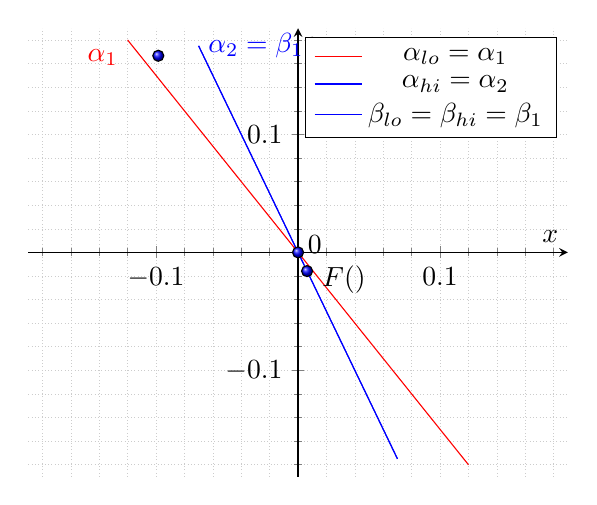
\begin{tikzpicture}
			\begin{axis}[
				axis lines=middle,
				xmin=-0.19,xmax=0.19,ymin=-0.19,ymax=0.19,
				xtick distance=0.1,
				ytick distance=0.1,
				minor tick num = 4,
				xlabel=$x$,
				ylabel=$y$,
				grid=both, 
				grid style={very thin,densely dotted,black!20}]
				\addplot [domain=0.12:-0.12,samples=2, color=red] {x*(-3)/2} node[below left]{$\alpha_1$};
				\addplot [domain=0.07:-0.07,samples=2, color=blue] {x*(-5)/2} node[right]{$\alpha_2 = \beta_1$};
				\addplot [domain=0.07:-0.07,samples=2, color=blue] {x*(-5)/2} node[right]{};
				
				\addlegendentry{$\alpha_{lo} = \alpha_1$}
				\addlegendentry{$\alpha_{hi} = \alpha_2$}		
				\addlegendentry{$\beta_{lo} = \beta_{hi} = \beta_1$}
				
				\addplot [
				only marks,
				mark=ball,
				mark size=2pt,
				point meta=explicit symbolic,
				nodes near coords,
				every node near coord/.append style={yshift=3pt,anchor=west},
				] coordinates {
					(-31/315,1/6) [$\eps$]
					(0,0)    [$\bm{0}$]
				};
			
				\addplot [
			only marks,
			mark=ball,
			mark size=2pt,
			point meta=explicit symbolic,
			nodes near coords,
			every node near coord/.append style={xshift=2pt,yshift=-3pt,anchor=west},
			] coordinates {
				(2/315, -1/63) [$F(\eps)$]
			};
			\end{axis}
		\end{tikzpicture}
	\end{center}
\caption{$\mdp_3$ illustrating case 4.b.i}
\label{fig:2d-plot}
\end{minipage}
\end{figure}
%%
\begin{example}\label{ex:2d}
	We provide an example~$\mdp_3$ with $d=2$,
	where $\eps, F(\eps)$ are vectors incomparable with~$\bm{0}$,
	and $F^2(\eps) = \bm{0}$.
	Here, $\alpha_1(x_1, x_2) = \frac{1}{2}x_1 + \frac{1}{3}x_2$, $\alpha_2(x_1,x_2) = \beta_1(x_1, x_2) = \frac{1}{2}x_1 +\frac{1}{5}x_2$.
	That is, the example fits into the Case~4b.i.
	Let $\eps = (-\frac{31}{315},\frac{1}{6})$. Then, $\alpha_1(\eps) > \alpha_2(\eps)$; we get~$F(\eps) = (\frac{2}{315},-\frac{1}{63})$.
	Further, $\alpha_2(F(\eps)) > \alpha_1(F(\eps))$ and $F^2(\eps) = (0,0)$.
\end{example}

